%!TEX root = ../thesis.tex
%*******************************************************************************
%*********************************** First Chapter *****************************
%*******************************************************************************

\chapter{An example of data-driven science}  %Title of the First Chapter
\label{chap:intro_stat}
\ifpdf
    \graphicspath{{Chapter1/Figs/Raster/}{Chapter1/Figs/PDF/}{Chapter1/Figs/}}
\else
    \graphicspath{{Chapter1/Figs/Vector/}{Chapter1/Figs/}}
\fi

\victor{This is a example of comment}

\cecile{This is a example of comment}

\isabelle{This is a example of comment}

\david{This is a example of comment}

\topic{This is a example of topic}
\content{This is a example of content}


\topic{Simulations combined with machine learning make possible to extract knowledge even in highly complex and stochastic process like High Energy Physics}

\content{Objective : Improving the precision of parameter estimation in a special case of the inverse problem in the presence of systematic effect.}


The first section (\autoref{sec:inverse_problem_at_lhc}) of this chapter describes the system and specific features of the analysis.
Then \autoref{sec:inference_through_simulation} provides methods to conduct the analysis in an ideal setup.
Finally the last parts of the analysis pipeline handling known biases and uncertainties are given in \autoref{sec:systematic_effects}.
\autoref{sec:summary} is gathering it all and emphasizes the part of the pipeline this work focus on.



\section{Inverse problem at LHC} % (fold)
\label{sec:inverse_problem_at_lhc}

% section inverse_problem_at_lhc (end)

\topic{C'est très complexe mais on a pas besoin de toute cette complexité pour saisir le problème.}





\subsection{The system} % (fold)
\label{sub:the_system}

The system producing the data studied in this analysis is the famous Large Hadron Collider (LHC).
Without getting into the details, a particle collider is a machine accelerating small bricks of matter, protons in this case, in opposite direction to smash them against each others.
The resulting collision produces high energy particles whose properties are captured by the various measurement apparatus which, for simplicity, can be reduced to a giant camera.

\victor{FIGURE : Utiliser des images + jolies}

\begin{figure}[htb]
    \centering
    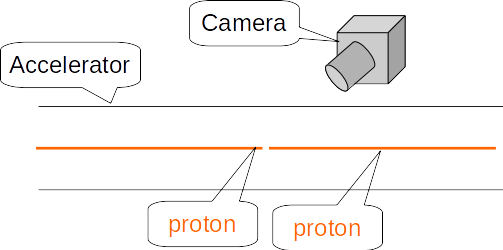
\includegraphics[width=0.8\linewidth]{particle_collider_0}
    \caption{Very simple particle collider}
    \label{fig:particle_collider_0}
\end{figure}


These collisions can be classified into 2 kinds :
\begin{itemize}
	\item the \emph{soft collisions} when the protons "missed" each other and does not produce high energy particles
	\item the \emph{hard collisions} when the protons smashed on each other and produces many particles
\end{itemize}

\begin{figure}[htb]
  \centering
  \begin{subfigure}[t]{0.49\linewidth}
    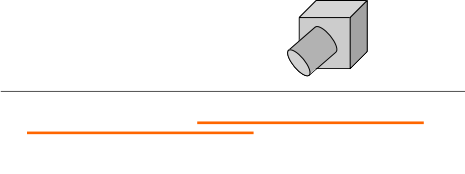
\includegraphics[width=\linewidth]{particle_collider_soft}
    \caption{soft collision}
    \label{fig:soft_collision}
  \end{subfigure}%
  \hfill
  \begin{subfigure}[t]{0.49\linewidth}
    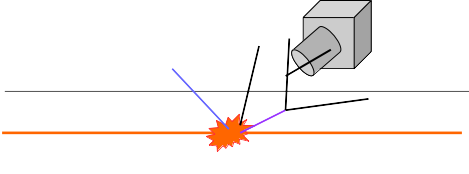
\includegraphics[width=\linewidth]{particle_collider_hard}
    \caption{hard collision}
    \label{fig:hard_collision}
  \end{subfigure}
  \caption{soft collision (left) and hard collision (right)}
  \label{fig:collision}
\end{figure}

The hard collisions, usually named \emph{event} in the High Energy Physics (HEP) community, are way rarer than the soft one.
The process creating the high energy particles is fundamentally stochastic.
Meaning that the nature and properties (eg. kinematics) of the process producing particles are not fully predictable but follow
probability distributions whose shapes and properties are deterministics.

The vast majority of the processes are already well known.
To produce (very) rare therefore interesting processes the accelerator must produce a collosal number of collisions.

The LHC is an international collaboration, involving thousands of people and housing many HEP experiments.
The one that motivates this work is a study of a specific process ($H \to \tau \tau$).
Basically an event produced a Higgs boson which desintegrated into 2 $\tau$ particles.
Each event following this process is defined as a \emph{signal} event versus the \emph{background} events that gather all the other processes.
The objective is to measure the frequency, or probability, of this event to occur.
Leading to a counting experiment of the number of signals $s$ and the number of backgrounds $b$ to estimate the quantity of interest $f = \frac{s}{s + b}$.
From this frequency and the setup of the experiment (luminosity, etc) it is possible to compute the \emph{cross-section} (or branch factor ?) of the $H \to \tau \tau$ process which is the final goal of the study.
\victor{Link between cross-section, branch factor, luminosity ?}

In many interesting cases, including ours, the nature of the event (signal / background) are not among the possible measurements that can be made.
Counting signals and backgrounds requires extra work which is described in this chapter.

The first step is to provide a very accurate description of the various steps in the experiment \ie the model.






\subsection{The model} % (fold)
\label{sub:the_model}

The Standard Model \needcite (SM) is the theory describing quantum physics including particle collisions and productions.
The counting experiment final objective is to improve our knowledge of one of the free parameter of the SM.
In other words we are fitting the SM parameters to the data of the experiment.

Let $x$ be the observables \ie the data collected by the apparatus for a single event and $p(x)$ its probability density.
The LHC produces a large quantity of events while ensuring that the conditions are the same for all events.
Hence we can assume that the full dataset $D$ contains $N$ independant and identically distributed (iid) events $D = \{x_i\}_{i=1}^N$.

Going from the fundamental parameters to the observables is very complex and not in the direct interest of this study.
The full process can be summaried into four major steps :
\begin{enumerate}
	\item The collision between particles
	\item The particle production from the collision
	\item The journey of the created particles to the apparatus (particle desintegrations into other particles, interactions between produced particles, etc)
	\item Reaction of the measurement apparatus to the particles going through it.
\end{enumerate}

Each of these steps requires special care from the community to be accurately modeled.
\victor{TODO : Maybe a few numbers to show how much it is complicated (nb poeple working on it, time required, nb of paper, etc)}

Although modeling what happens between the particle production and the apparatus response is possible it is by definition impossible to get data about what really happened.
Leading to the necessity to infer what happened before the measurements.

\victor{TODO : Quelques mots sur le tracking, l'inférence des features}

The vast majority of the intermediate quantities are latent or hidden variables, noted $z$.
One of this latent variable was already mentioned previously : the \emph{label} of the event indicating the nature of the process, in our case if it is a \emph{signal} or a \emph{background} event.

\victor{L'objectif est de donner un apperçu de la complexité de la chose. Sans entrer + que ça dans les détails...}
\victor{TODO : Donner un aperçu de la complexité de chaque étape en 1 ou 2 phrases.}

In this study the parameter of interest, noted $\mu$, is a fundamental parameter intervening at the particle collision stage (ie step 1).

Finally gathering all the ingredients the generative model can be splited in 3 stages :
\begin{equation}
	\label{eq:model_simple}
	p(x, \mu, z) = p(x|z) p(z | \mu) p(\mu)
\end{equation}
In other words the fundamental parameter $\mu$ shapes the distribution of the latent variable $z$.
And the data distribution depends on the latent variable $z$.
$p(\mu)$ is the prior knowledge, it contains all the belief of the community.
Of course the belief of the community is only based on results of previous experiments or non-informative if there is no previous experiments.

Note : we assume here that $\mu$ is the only fundamental parameter for simplicity.
In a more realistic model, like the standard model, there are more fundamental parameters.
To these fundamental parameters one should also take into account the parameters intervening in the apparatus response modeling.
Additionally some required model simplifications introduce again some parameters, etc.
How to take care of these additional parameters is the subject of \autoref{sec:systematic_effects}.

The true value of $\mu$, assuming that the model is perfectly describing Nature's behaviour, is noted $\mu^\star$ as opposed to $\hmu$ the estimated value from the data.
Of course the objective is to build an estimator $\hmu$ whose value is as close as possible to the true value $\mu^\star$.







\subsection{Classic parameter estimation} % (fold)
\label{sub:classic_parameter_estimation}

\topic{Bayesian inference gives access to the full posterior distribution}


Assuming that the model provides a likelihood $p(x | \mu)$ the Bayes theorem indicates how to access the posterior pobability.
\begin{equation}	
    p(\mu | x) = \frac{p(x|\mu) p(\mu)}{p(x)} = \frac{p(x|\mu) p(\mu)}{\int_\mu p(x|\mu) p(\mu)}
\end{equation}

The prior $p(\mu)$ contains all the current knowledge about the parameter. 
If no knowledge is available a non informative prior is chosen, usually a uniform distribution over the domain of $\mu$.
The inference is then straitforward.
Computing $p(\mu | x)$ for the possible values $\mu$ \ie where the prior probability is not zero.
The integral on the denominator can either be computed by hand or approximated with Monte Carlo.

Often the full posterior is not required and only the most probable value of the parameter is infered.
When no prior knowledge on the parameter of interest is available maximum a posteriori and maximum likelihood estimators are strickly equivalent.
\begin{align}
	\argmax_\mu p(\mu | x) &= \argmax_\mu p(\mu | x) \\
							&= \argmax_\mu \frac{p(x|\mu) p(\mu)}{p(x)} \\
							&= \argmax_\mu p(x|\mu) p(\mu) \\
							&= \argmax_\mu p(x|\mu)\\
\end{align}
Solving this maximization usually involves either analytical computing of the formulas \victor{Why not givin an example in the appendix ?} or a numerical optimization process (eg. gradient ascent, coordinate ascent)








\subsection{Inverse problem} % (fold)
\label{sub:inverse_problem}

\topic{These methods don't scale to high dimensions}

Unfortunately the likelihood provided by the model is not tracktable.
The process leading from the collisions to the obvervables involves numerous latent variables $z_1, ..., z_n$ where $n=10^6$.
Making the marginal likelihood intraclable because of high dimensional integrals.
\begin{equation}
	\label{eq:intractable_integral}
	p(x|\mu) = \int_{z_1} \int_{z_2} ... \int_{z_n} p(x|\mu, z_1, z_2, ..., z_n) p(z_1) p(z_2) ... p(z_n)
\end{equation}

\victor{What do we know about numerical stability of high dimensional integral ?}
\content{Maybe a "simple" example that shows how often in real life this setting may happen}

Moreover sometimes simplifications needs to be made in order to build the model \needcite making the computed likelihood only a approximation of the true likelihood.
Some other times computable formulas simply do not exist \needcite.

\content{Approximation requiered to build some part of LHC simulation as an example}


However building a simulator working only in forward mode ie allowing to sample from $p(x|\mu)$ is easier and possible in cour case.
The objective is then to infer causal parameters from observations hence reversing the forward process which goes from causal parameters to observations.
This is more generaly known as the \emph{inverse problem}.
There is no general solution yet to this problem altough it occures often in experimental science.


\begin{figure}[htb]
    \centering
    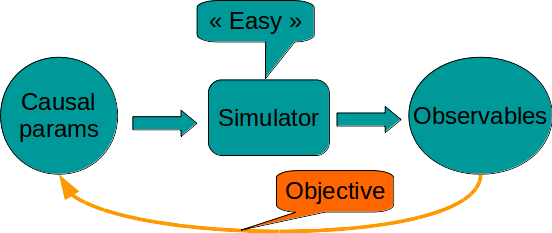
\includegraphics[width=0.8\linewidth]{inverse_problem}
    \caption{The inverse problem objective is to go from the observables to the causal parameter of the model embeded by the simulator}
    \label{fig:inverse_problem}
\end{figure}



\subsection{Special case of inverse problem} % (fold)
\label{sub:special_case_of_inverse_problem}

Although no general solution to the inverse problem exist yet it is possible to use the characteritics of the setup to get around the problem.

Events are classified into two categories : signals and backgrounds.
The distribution of events can be rewritten as :
\begin{equation}
 	p(x) = p(x|S) p(S) + p(x|B) p(B)
\end{equation}
The objective is to infer the probability of an event to be a signal ie $p(S)$ while $p(x|S)$ and $p(x|B)$ are intracktable.
Since we are working with very rare events the value of $p(S)$ is very small.
To avoid numerical issues it is more convenient to deal with a \emph{deviation} from a nominal value.
\begin{equation}
	p(S) = \mu p_{SM}(S)
\end{equation}
where $p_{SM}(S)$ is the probability of an event to be a signal according to current knowledge ie the Standard Model.
The parameter of interest $\mu$ is measuring the deviation of the data from the SM.
If the data are in perfect agreement with the SM then $\mu=1$.

The next section will make use of this setup to tackle the inference.






\section{Inference through simulation} % (fold)
\label{sec:inference_through_simulation}

\victor{Or "Inference with/using simulations" ?}

\topic{Simulations/models are useful to explain data (therefore understand the undelying process that generated the data)}


\content{Dans un monde simple tout est "facile"}
\content{Introduire le problème d'extraction d'un coefficient de mélange(lié à cross-section)}


This section show how to solve this specific case of inverse problem.
\autoref{sub:hand_crafted_dimension_reduction} gives a general solution assuming domain knowledge allow to put all relevant information in a low dimension space.
\autoref{sub:count_estimation} is using a classifier score as a proxy for maximum likelihood estimation.
The remaining sections (\autoref{sub:poisson_count_process}, \autoref{sub:binned_poisson_count_process}, \autoref{sub:asimov_dataset}) describe the retained analysis pipeline.
The reason to retain the last one is given in \autoref{sec:systematic_effects}.









\subsection{Hand crafted dimension reduction} % (fold)
\label{sub:hand_crafted_dimension_reduction}

\victor{Brouillon}

Since the likelihood cannot be computed directly one solution is to sample many events and apply density estimation methods.
Examples : histograms, kernel density estimation.
Tackling the inverse problem with density estimation is subject to the curse of dimensionality.
Restricting the observables to only one or two dimensions requires those dimension to carry all or most the information about the estimated parameter.

The first idea to achieve such constraint is to use domain knowledge.
Basically ask the theorist to find a computable quantity from the possible measurement allowing to infer the parameter.
\victor{TODO : Fouiller les années 80 à la recherche d'exemple}

\victor{Discard the less relevant ones (feature selection). Pas sûr que ça soit vraiment utilisé. Demander à David.}

The second possibility is to use machine learning to reduce the dimension of the data.


\victor{Parzen windows to estimated density to get a likelihood. Maybe beats curse of dimension.}
Parzen windows can estimate densities !
So we can use it on the simulated data to define the likelihood function.

\victor{Mot clé : "méthode des coupures" (cécile) comme méthode à la main pour trouver une région riche en signal}







\subsection{Count estimation} % (fold)
\label{sub:count_estimation}

This section borrows many results from \cite{Neal:2007zz}.

The stochastic phenomenon of interest here displays the following generative process :
\begin{equation}
	\label{eq:mixture_model}
	p(x|\eta) = \eta p(x|S) + (1-\eta) p(x|B)
\end{equation}
where $x$ is the set of observable features of the studied event gathered in a vector.
Events are split into 2 classes : the signals $S$ and the backgrounds $B$.
Note that $S$ and $B$ are one of the numerous latent variable $z_i$ in \autoref{eq:intractable_integral}.
$\eta$ is the mixture coefficient between signals and backgrounds.

As stated in \autoref{sub:special_case_of_inverse_problem} $\eta$ can be seen as the probability for an event to be a signal $p(S)$. 
It naturally follows that $1-\eta$ is the probability for an event to be a background $p(B)=1-p(S)$.
\autoref{eq:mixture_model} can be re-written as
\begin{equation}
	p(x) = p(S)p(x|S) + p(B)p(x|B)
\end{equation}

As previously explained \autoref{sub:inverse_problem} the likelihoods $p(x|S)$ and $p(x|B)$ are intractable because they involves high dimension integrals.
However building a simulator working only in forward mode allowing to sample from $p(x|\eta)$ is possible.
This allow us to build a training dataset to feed some machine learning algorithm later.

Measurements are made from a large bunch of independent and identically distributed events $D=\{x_i\}_{i=1}^N$.

\begin{align*}
	p(D|\eta) =& \prod_{i=1}^N \eta p(x|S) + (1-\eta) p(x|B) \\
	       =& \prod_{i=1}^N p(x|B) \left [(1-\eta) + \eta \frac{p(x|S)}{p(x|B)} \right ]\\
\label{eq:Fisher-Neyman}
	       =& \underbrace{\left[ \prod_{i=1}^N p(x|B) \right ]}_{h(x)} \times 
	       \underbrace{\left [\prod_{i=1}^N (1-\eta) + \eta \frac{p(x|S)}{p(x|B)} \right ]}_{g_\eta(T(x))}
\end{align*}
with $T(x) = \frac{p(x|S)}{p(x|B)} $

The Fisher-Neyman factorization theorem \needcite states that $T(x)$ is a sufficient summary statistic to obtain $\eta$

The maximum likelihood estimator, noted $\hat \mu$, is commonly used to estimate the parameter of interest.
This is a reasonable choice when we do not have prior knowledge as in this example.

\begin{equation}
	\hat \eta = \argmax_\eta p(\eta | D)
\end{equation}

It is more convenient (numerical stability) to express the result as a deviation from the prediction of the Standard Model.
The deviation is defined as :

\begin{equation}
	\mu = \frac{p(S)}{p_{SM}(S)} = \frac{\eta}{p_{SM}(S)}
\end{equation}
$p_{SM}(S)$ is the expected probability to get a signal following the Standard Model.
Recovering the frequency $\eta$ from $\mu$ is trivially done with $\eta = \mu p_{SM}(S)$.

The estimator is now :
\begin{align}
	\hmu =& \argmax_\mu  p(D | \mu) \\
	     =& \argmax_\mu  \prod_{i=1}^N g_\mu(T(x)) \\
\end{align}


$T(x)$ can be obtained using a classifier $c$ trained to separate signals and backgrounds.
A Bayes optimal classifier output gives :
\begin{equation}
	c(x) = \frac{n_s p(x|S)}{(1-n_s) p(x|B) + n_s p(x|S)}
\end{equation}
where $n_s$ is the fraction of signals used in the training dataset.

\begin{equation}
	T(x) = \frac{c(x)}{(1-c(x))} \frac{(1-n_s)}{n_s} 
\end{equation}


Note that $c$ is also a sufficient summary statistic
\begin{equation}
	g_\mu(T(x)) = 1 - \mu p_{SM}(S) + \mu p_{SM}(S) \times \frac{c(x)}{(1-c(x))} \frac{(1-n_s)}{n_s} = f_\mu(c(x))
\end{equation}

\content{Limitation : what happens if the classifier is not (Bayes) optimal ? Can we detect it ?}
\content{Physicists also uses the Neyman-Pearson theorem on statistical test to justify maximum likelihood estimator usage. Should I include it here ?}

\victor{TODO : C'est ici que je devrais parler des travaux de Kyle Cranmer et al sur Calibrated classifier ! \cite{Cranmer2015}}










\subsection{Poisson count process} % (fold)
\label{sub:poisson_count_process}

Here is derived the standard method to solve the problem.
The modeling of events is replaced by a model at a dataset level which is tractable.

The system allows 2 kind of collisions : soft and hard collisions.
The hard collisions are very rare compared to the soft collisions.
The data can be modeled by counting iid Bernoulli rare process which is well approximated by a Poisson distribution \needcite when the number of samples is large.

\victor{FIGURE : Ajouter un petit dessin type arbre de probabilité.}

The hard collision are splitted into 2 categories the signal events and the background events.
The number of signals is $s$ and the number of backgrounds is $b$.

The total number of events $n$ is the sum of signal events and background events.
\begin{equation}
	n = s + b
\end{equation}
The number of signal events is following a Poisson distribution of parameter $\mu \gamma$.
\begin{equation}
	s \sim Poisson(\mu \gamma)
\end{equation}
$\gamma$ is the expected number of signals according to current knowledge ie the SM.
$\mu$ is the parameter of interest, it is the deviation from the SM.
This way of decomposing the expectancy of the number of signals is mainly here for convenience : numerical stability ($\gamma$ is of the order $10^-6$\needcite; and dimensionless $\mu$.
\victor{dimensionless or unitless ?}
The number of background events is following a Poisson distribution of parameter $\beta$.
\begin{equation}
	b \sim Poisson(\beta)
\end{equation}
Since the sum of Poisson random variables is also Poisson distributed \needcite (cf wikipedia) :
\begin{equation}
	n \sim Poisson(\mu \gamma + \beta)
\end{equation}

Giving the likelihood :
\begin{equation}
	P(n| \mu) = \frac{(\mu \gamma +\beta)^n }{n!} e^{-(\mu \gamma +\beta)}
\end{equation}

A tractable likelihood is now available !
This allow to use more classic parameter estimation like maximum likelihood.

\begin{equation}
    \hat \mu = \argmax_\mu p(n|\mu) =  \argmax_\mu Poisson(n|\mu)
\end{equation}
This can be done by hand. Assuming that we know $\gamma$ and  $\beta$.
\begin{equation}
    \frac{\partial \log p(n|\mu)}{\partial \mu} =  \gamma \frac{n}{\mu\gamma + \beta} - \gamma
\end{equation}
\begin{equation}
    \frac{\partial \log p(n|\mu)}{\partial \mu} = 0 \iff \mu = \frac{n-\beta}{\gamma}
\end{equation}
Note $\EE[n] = \mu\gamma + \beta$ and $\max Poisson = \EE[Poisson]$ so maybe there is a simpler way to find this ?






\subsection{Binned Poisson count process} % (fold)
\label{sub:binned_poisson_count_process}

The previous section gives a simple way to derive a maximum likelihood estimator.
This section show how to improve this estimator using binning.

The Poisson approximation is allowed because of the small probability of a event to occur and the large number of samples that the LHC can produce.
Cutting the data space into regions does not break these assumptions as long as the regions contains enough samples.
Intuitively knowing not only the total number of events but the number of events in each chunk of the data space contains more information hence should improve the inference.

Let $O$ be the full data space and $K$ regions $\{\Omega_i\}_{i=1}^K$ such that they do not overlap $\forall i\neq j, \Omega_i \cap \Omega_j = \varnothing $ and that their union cover the full space $\bigcup_{i=1}^K \Omega_i = O$.
Those regions are most commonly called \emph{bins} (or histogram bins) as the counting events in regions often rely on building a histogram.

There is an infinite number of ways to cut the space into bins.
\victor{FIGURE : Dessin de 2 manières de couper l'espace en région}
Our objective with the binning is to improve the estimation, especially reduce the variance of our estimator.

First let's see how binning improves the variance.
We compare the two likelihood functions $L_0$ without binning and $L_K$ with $K$ bins
\begin{equation}
    L_0 = \frac{(\mu \gamma + \beta)^n }{n!} e^{-(\mu \gamma + \beta)}
\end{equation}
with $n = \sum_{i=1}^K n_i $, $\gamma = \sum_{i=1}^K \gamma_i $ and $\beta = \sum_{i=1}^K \beta_i $.
\begin{equation}
    L_K = \prod_{i=1}^M \frac{(\mu \gamma_i + \beta_i)^{n_i} }{n_i!} e^{-(\mu \gamma_i + \beta_i)}
\end{equation}

$L_0 > L_K$ and 
$\left (\frac{\partial^2 \log L_0}{\partial \mu^2}\right )^{-1} > \left (\frac{\partial^2 \log L_K}{\partial \mu^2}\right )^{-1}$.
See \autoref{sec:proof} for details of the proof.

According to the Cramer-Rao bound :
\begin{equation}
    \VV(\hmu) \geq \left (\frac{\partial^2 \log L}{\partial \mu^2}\right )^{-1}
\end{equation}

If the bound is tight the binned likelihood $L_K$ leads to a estimator with lower variance.
If the bound is not tight well it is still probably better.

The choice of the bin shape remains to be decided.
\begin{equation}
    \left (\frac{\partial^2 \log L}{\partial \mu^2}\right )^{-1} = \left ( \sum_{i=1}^K n_i \frac{\gamma_i^2}{(\mu \gamma_i + \beta_i)^2} \right )^{-1}
\end{equation}
Choosing carefully the bins $\Omega_i$ to make this quantity as small as possible requires to have some bins with high purity of signals.
\victor{I need to prove that ! See \autoref{sec:proof} for details}

To improve inference a classifier is used to create at least one region as rich in signals as possible.
As seen in \autoref{sub:count_estimation} a Bayes optimal classifier decision function is a sufficient summary statistic adding to the interest of using a classifier.








\subsection{Asimov dataset} % (fold)
\label{sub:asimov_dataset}

This section deals with the estimation of $\gamma_i$ and $\beta_i$ using the simulator.

\victor{Brouillon}

Basically we want $\gamma_i = \EE [s_i]$ and $\beta_i = \EE [b_i]$.
We could estimate $\EE [s_i]$ and $\EE [b_i]$ by Monte Carlo.
And I remember that the Asimov dataset is a dataset whose properties are equals to their expectancy.
In the code I am estimating $\EE [s_i]$ and $\EE [s_i]$ by putting a simulated dataset through the entire pipeline.
So I guess that it is not that complicated after all.

\victor{PAPER : trouver les papiers de référence ou les papier tuto pour Asimov dataset}








\section{Systematic effects} % (fold)
\label{sec:systematic_effects}

\topic{Systematic effects make inference more complex by introducing nuisance parameters}

The parameter of interest is not the only causal parameter in real life experiments.
Many other parameters are required to explain the observed data.
Here is described the methods to take into account those additional parameters and their impact on inference. 





\subsection{Definition} % (fold)
\label{sub:definition}

Real life data modeling often requires several parameters to be fully described.
On the other hand only one or a few of these parameters are the object of one study.
This leads to asign parameters into two classes : the parameter of interest and the nuisance parameters.

Nuisance parameters can appear from :
\begin{itemize}
	\item apparatus imperfections
	\item theory flaws
	\item fundamental parameter uncertainties
	\item etc
\end{itemize}

Here is an example to 
Bob wants to estimate the efficiency of its hotplate by measuring the time required to heat 1L of water in a saucepan to boiling temperature.
Each time Bob need boiling water to cook he will run this little experiment.
Bob measured the temperature of the water and the air and the air pressure and know the electric power of his hotplate.
Unfortunatelly Bob is using tap water and cannot measure the amount of impurities in the water which have a influence on the boiling temperature.
The impurities concentration in the water is now a nuisance parameter of the problem (fundamental uncertainty).
Moreover the thermometer is a cheap one and may be biased toward lower or upper temperature introducing another nuisance parameter (apparatus imperfection).
Finally to simplify the computation Bob assumed that the heat produced by the hotplate would be mostly transmitted to the water.
Although this approximation is too strong Bob will take it into account with a simplified formulas involving an additionnal nuisance parameter (theory flaws).

\content{FIGURE : Schéma inverse problem with nuisance parameters}

In the remaining of this manuscript the nuisance parameters are all gathered into a vector $\alpha$.




\subsection{Impact on likelihood} % (fold)
\label{sub:impact_on_likelihood}

\victor{Brouillon pour le moment}

First, the introduction of nuisance parameters $\alpha$ in \autoref{eq:Fisher-Neyman} makes it impossible to use the Fisher-Neyman theorem.
\begin{equation}
	p(D|\mu, \alpha) = \underbrace{\left[ \prod_{i=1}^N p(x|B, \alpha) \right ]}_{h_\alpha(x)} \times 
       \underbrace{\left [\prod_{i=1}^N (1-\mu) + \mu \frac{p(x|S, \alpha)}{p(x|B, \alpha)} \right ]}_{g_\mu(T_\alpha(x))}
\end{equation}
Now $h_\alpha(x)$ does not depends only in $x$.
One could argue that although the classifier score may not be a sufficient summary statistic anymore it is probable that it still contains most of the information about the parameter of interest.

The use of classifier score is a very good approximated proxy to the likelihood function in practice.
Moreover \cite{Cranmer2015} shows that if the classifier score is a monotone function of the likelihood it is a sufficient statistic.
\victor{TODO : vérifier les termes exact du théorème de Cranmer}

Second, the poisson count likelihood (see \autoref{sub:poisson_count_process}) has to be updated with the introduction of the nuisance parameter $\alpha$.
The expected number of signal $\gamma$ and backgrounds $\beta$ now depends on $\alpha$.

\begin{equation}
	P(n| \mu, \alpha) = \frac{(\mu \gamma(\alpha) +\beta(\alpha))^n }{n!} e^{-(\mu \gamma(\alpha) +\beta(\alpha))}
\end{equation}

Which makes it impossible to use closed formulas since these dependencies are not known exactly or intractable.
Moreover taking nuisance parameter into account can introduce local maxima in the likelihood function.

\victor{TODO : C'est là que j'attaque les papiers avec linéarisation de l'impact du paramètre de nuisance}

$\alpha$ is generally known to a certain extent thanks to other measurements is controlled region where the signal has low probability of appearing or even no influence at all making these measurement independent from $\mu$.

These measurements $D_{calib}$ very often constrains the values of $\alpha$ with a gaussian distribution :
\begin{align}
	p(n, D_{calib} | \mu, \alpha) &= p(n | \mu, \alpha) \times p(D_{calib} | \mu, \alpha) \\
	p(n, D_{calib} | \mu, \alpha) &= p(n | \mu, \alpha) \times p(D_{calib} | \alpha) \\
	p(n, D_{calib} | \mu, \alpha) &= Poisson(n | \mu \gamma(\alpha) +\beta(\alpha)) \times \mathcal N(D_{calib} | \alpha)
\end{align}

Of course this can be extended to the binned poisson likelihood.
\begin{equation}
	p(n_1, .., n_K, D_{calib} | \mu, \alpha) = \mathcal N(D_{calib} | \alpha) \times \prod_{i=1}^K Poisson(n_i | \mu \gamma_i(\alpha) +\beta_i(\alpha))
\end{equation}





\subsection{Classifier optimality} % (fold)
\label{sub:classifier_optimality}


\victor{Brouillon}







\subsection{Recipes to reduce systematic uncertainties} % (fold)
\label{sub:recipes_to_reduce_systematic_unceratinties}

\victor{Brouillon}

Petite listes des choses faisables pour réduire les biais systématiques. 


Example : Calibrant interne en chimie (mesure supplémentaire dont la valeur attendu est connu). Calibrant externe (échantillon dont la valeur attendu est connu).








\subsection{Variance estimations} % (fold)
\label{sub:variance_estimations}

\victor{Brouillon}

For now the concerns were mostly focused the inference of the parameter.
But this is only half the answer.
In science every estimation must comes with its uncertainty.
The other half is the measurement of the uncertainty of parameter of interest's estimator.

The origin of the variance of our estimator can be divided into 2 parts.
The one comming mostly from the lack of data is called \emph{statistical variance} and the other origniates from the sensitivity of the inference to nuisance parameter and is named \emph{systematic variance}.

Reminder of the variance definition :
\begin{equation}
	\VV(Y) = \EE[(Y - \EE[Y])^2] = \EE(Y^2) - [\EE(Y)]^2
\end{equation}

Law of total variance \needcite :
\begin{eqnarray}
\label{eq:total_variance_law}
    \VV[Y] =& \EE_X \left (\VV[Y|X] \right ) &+ \VV_X \left (\EE[Y|X]\right ) \\
    \VV[Y] =& \EE_X \left (\VV[Y|X] \right ) &+ \EE_X \left ( (\EE [Y|X]  - \EE[Y])^2\right )
\end{eqnarray}


Substituing with our problem the estimator $Y = \hmu$ and the nuisance parameter $X = \alpha$ :

\begin{equation}
\label{eq:stat_and_syst_variance_definition}
\mathbb{V}[\hmu] 
	= \underbrace{\mathbb{E}_{\alpha \sim p(\alpha)} \left (\mathbb{V}[\hmu | \alpha] \right )}_{V_{stat}} 
	+ \underbrace{\mathbb{E}_{\alpha \sim p(\alpha)} \left ( (\mathbb{E} [\hmu | \alpha]  - \mathbb{E}[\hmu])^2\right )}_{V_{syst}}
\end{equation}

The variance of our estimator is splitted into :
the average of the variances of our estimator (assuming $\alpha$ is known) and the deviation from the average estimator induced by the nuisance parameter.

\victor{Voilà c'est bien joli, mais il reste des zones d'ombre. c'est quoi $p(\alpha)$ ? et c'est quoi $\hmu | \alpha$ ?}

Is the following correct ?
\begin{align}
	\hmu | \alpha &= \argmax_{\mu, \alpha} p(Data | \mu, \alpha) | \alpha \\
		&= \argmax_{\mu} p(Data , \alpha | \mu)
\end{align}

Obviously $p(\alpha)$ is a prior distribution.
If the likelihood already includes calibration then it simply should represent the community's belief (without data) on the nuisance parameters.





\subsection{Profiled likelihood} % (fold)
\label{sub:profiled_likelihood}

\topic{The current way of measuring the variance of our estimation to include systematics is "profiled likelihood"}

\content{Explain how profiled likelihood works and why is works}
\content{Introduce Fisher information matrix and Cramer Rao bound (since we will use it later for INFERNO)}


references : 
\begin{itemize}
	\item \url{https://arxiv.org/abs/physics/0403059}
	\item \url{https://arxiv.org/abs/1007.1727}
	\item \url{https://arxiv.org/abs/physics/0408039} coverage study of marginalization of nuisance params
\end{itemize}

\content{Expliquer pourquoi on a pas de formule close form pour}



Il s'agit de produire $\mu$ et de l'encadrer.
Version simple : Monte Carlo pour avoir p(x) et chercher le maximum.

Puis pour l'encadrement on navigue autour du maximum pour obtenir à droite et à gauche la valeure qui corespond à l'encadrement.
On veut un interval de confiance à X\%.
On va faire des petits calculs + petites approximations pour mesurer la valeur de $\mu + \smu$ et de $\mu - \smu$.


\content{Faire un petit examle à la main end-to-end}
\content{Lister clairement les approximations faites pour obtenir cet intervalle de confiance. + citer les papiers qui ont challengé ces apprixmation }





\section{Summary} % (fold)
\label{sec:summary}


\subsection{Workflow} % (fold)
\label{sub:workflow}

\victor{En fait qu'est-ce que je veux dire ici ?}

In practice the data go through many processes like trigger selection, tracking, event reconstructions, etc computing hand crafted features to reduce the dimensionality from $\RR^{100,000}$ to $\RR^{40}$ then using machine learning to reduce to $\RR$.
Although machine learning is slowly becoming part of these steps \needcite.
All the domain knowledge is concentrated in the simulator and the hand crafted data processing.


\begin{figure}[htb]
    \centering
    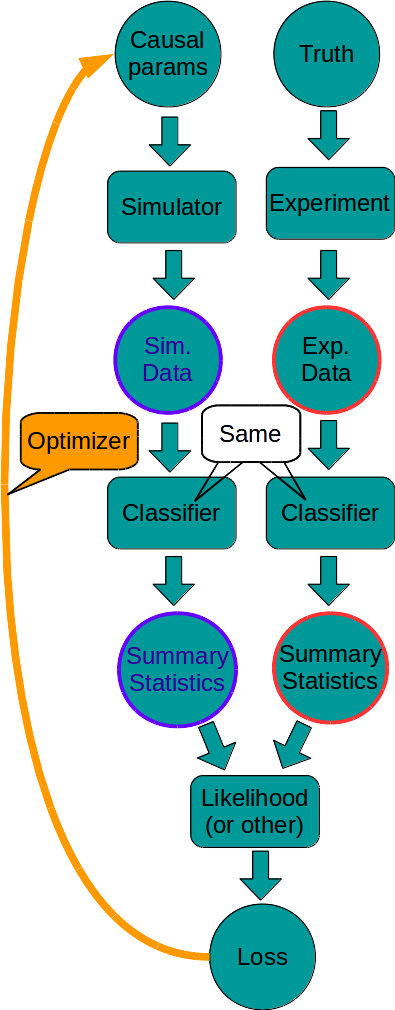
\includegraphics[width=0.5\linewidth]{workflow}
    \caption{The workflow of maximum likelihood inference using an optimizer}
    \label{fig:workflow}
\end{figure}


\victor{Papier de référence pour la construction d'interval de confiance en HEP = \url{https://arxiv.org/pdf/physics/9711021.pdf} G. J. Feldman and R. D. Cousins, Phys. Rev. D 57, 3873 (1998) ?}



\subsection{Looking for better} % (fold)
\label{sub:looking_for_better}

\topic{This document is about going further than the "simple" classifier method}

\content{Annonce de la suite / du plan du manuscrit}


